
\documentclass[runningheads,a4paper]{uwsese}

%ACHTUNG: Diesen Import für englische Arbeiten entfernen.
\usepackage[ngerman]{babel}

\usepackage[utf8]{inputenc}
\usepackage{amssymb}
\usepackage{amsmath}
\setcounter{tocdepth}{3}
\usepackage{graphicx}
\usepackage{array}
\usepackage{ragged2e}
\usepackage{arydshln}
\newcolumntype{P}[1]{>{\RaggedRight\hspace{0pt}}p{#1}}
%\newcolumntype{P}[1]{>{\raggedright\arraybackslash}p{#1}}


\usepackage{url}
\urldef{\mailsa}\path|maximilian.stock@stud-mail.uni-wuerzburg.de|
\newcommand{\keywords}[1]{\par\addvspace\baselineskip
\noindent\keywordname\enspace\ignorespaces#1}

\begin{document}

\mainmatter

% first the title is needed
\title{Konfigurationsmanagementstrategien und Tools in der SW Entwicklung:\\ Überblick und Beispiel}

% a short form should be given in case it is too long for the running head
\titlerunning{Konfigurationsmanagementstrategien und Tools}

\author{
  Maximilian Stock\\
  \texttt{maximilian.stock@stud-mail.uni-wuerzburg.de}\\
  \and\\
  Michael Steininger\\
  \texttt{michael.steininger@stud-mai.uni-wuerzburg.de}
}
%
%\authorrunning{Maximilian Stock}
% (feature abused for this document to repeat the title also on left hand pages)

% the affiliations are given next
\institute{Julius-Maximilians-Universität,
Würzburg\\
%\mailsa\\
}


% \toctitle{Interpolation based Modelling of Power and Performance}
% \tocauthor{J. von Kistowski and S. Kounevs}
\maketitle


\begin{abstract}
	Hier kommt der Abstract hin. Der Abstract behandelt alle Unterpunkte, welche auch in der Introduction behandelt werden (s. Section~\ref{sub:intro}) und liefert damit eine Zusammenfassung über die Seminararbeit als Ganzes. Im Gegensatz zur Zusammenfassung ist der Abstract sehr kurz gehalten und hat ca. ein bis zwei Sätze pro Unterpunkt.
\end{abstract}


\section{Einführung}
Ursprünglich ist die Idee des Konfigurationsmanagements im US-Militär
entstanden. Dort wurden in den 1950er Jahren Versuche mit Flugkörpern gemacht,
die in verschiedenen Konfigurationen gebaut und getestet worden sind. Eine
Vielzahl der Flugkörper sind nicht wie vorgesehen im Ziel explodiert sondern
meist zuvor. Es war allerdings nicht möglich die fehlerhaften Flugkörper nach
den Tests zu untersuchen, weil sie zerstört worden sind. Zusätzlich waren die
Aufzeichnungen über die Konfigurationen der einzelnen Flugkörper nicht
ausreichend. Dadurch war es nicht möglich festzustellen welche Änderungen zu
welchen Testausgängen führten. Aus diesen Erfahrungen enstanden
Konfigurationsmanagementstandards, die bei allen Änderungen eines Erzeugnisses
auch eine Änderung der Dokumente fordern.

Diese Probleme lassen sich analog auch in der Softwareentwicklung beobachten.
Es gibt z. B. Probleme durch undokumentierte Änderungen von Code oder
kurzfristige Änderungen am Quellcode vor
Auslieferung. Deshalb ist das Konfigurationsmanagement Teil von vielen
Reifegradmodellen wie z. B. {\em CMMI} oder
{\em SPICE}~\cite{weischedel2002}.

TODO: Aufbau der Arbeit

\section{Grundlagen}

\section{Software}

\section{Fazit}

\subsection{Allgemeiner Aufbau}

\textbf{Prinzip der Pyramide}: Der Aufbau eines wissenschaftlichen Papiers (und auch der Seminararbeit) sollte idealerweise dem Prinzip der Pyramide folgen. Das bedeutet, dass der Artikel einen hierarchischen Aufbau verfolgen sollte. Der eigentliche Inhalt des Papiers (Motivation, Inhalt, Ergebnisse) wird in mehreren Iterationen wiedergegeben (z.B. 3), wobei der Abstraktionsgrad bei jeder Iteration sinkt. In hochwertigen Publikationen (z.B. Papieren in IEEE TSE) ist dieses Prinzip deutlich zu erkennen. Dieses Prinzip wird bereits durch Abstract/Introduction induziert und sollte auch im Rest des Papiers weitergeführt werden. Der Vorteil ist, dass es das Verständnis eines komplexen Sachverhalts mit vielen Details wesentlich erleichtert, weil man die Struktur des Vorgestellten besser nachvollziehen kann. Der Leser kann die Details eines Lösungsansatzes besser einordnen, wenn er das Ziel der Argumentation bereits kennt. Auf diese Weise wird auch verhindert, dass ein Papier einen Krimi erzählt, bei dem erst am Schluss klar wird, worauf die Autoren hinaus wollten und was das eigentliche Ergebnis der Arbeit war.

\subsection{Über die Introduction}
\label{sub:intro}

``Abstract'', ``Introduction'' und ``Conclusions'' gehören zu den meist gelesenen Abschnitten eines Papers und sollten daher mit besonderer Sorgfalt geschrieben werden. Idealerweise enthalten Abstract und Introduction die folgenden 5 Punkte. In einem Abstract sollten zu jedem dieser Punkte ein bis zwei Sätze geschrieben werden, mehr nicht. Die Einleitung behandelt die gleichen Punkte, wie der Abstract, verwendet aber nicht nur ein bis zwei Sätze sondern ein bis zwei Absätze pro Punkt. Die Punkte sind:

\begin{enumerate}
	\item Eingrenzung des Forschungsbereichs (In welchem Themengebiet ist das Thema/die Arbeit angesiedelt?)
	\item Beschreibung des Problems, das in den bearbeiteten Arbeiten gelöst werden sollte (Was ist das Problem und warum ist es wichtig dies zu lösen?)
	\item Lösungsansatz/Lösungsansätze der zu bearbeitenden Arbeiten (Welcher Ansatz wurde in welcher Arbeit verwendet, um das Problem zu lösen? Was ist der Beitrag der jeweiligen Artikel?)
	\item Art der Validierung + Ergebnisse (Wie wurde nachgewiesen, dass die Arbeiten die versprochene Verbesserung wirklich vollbracht haben (Fallstudie, Experiment, o.ä.); Was waren die Ergebnisse der Validierung (idealerweise Prozentsatz der Verbesserung)?)
\end{enumerate}

 Die Einleitung dient dazu, den Leser an die Arbeit heranzuführen. Sie sollte sich von allgemeinen Aussagen zum eigentlichen Thema heranarbeiten (hineinzoomen). Die Einleitung sollte so geschrieben werden, dass jeder Informatiker (auch aus anderen Teilbereichen der Informatik) verstehen kann wozu die Arbeit dient. Idealerweise folgt die Einleitung dem gleichen Aufbau (5 Punkte) wie der Abstract, jedoch wird jetzt für jeden der Punkte ein ganzer Abschnitt geschrieben. Der vorletzte Absatz der Einleitung (also nach Abhandlung der 5 Punkte) sollte die Beiträge (Contributions) der bearbeiteten Werke nochmals deutlich herausstellen. Das erleichtert es Lesern, im Wust von Motivation, verwandten Arbeiten, Grundlagen usw. das Inkrement bzw. den wissenschaftlichen Beitrag der Arbeiten zu erfassen.

Im Allgemeinen schließt die Einleitung am Ende mit einer Mini-Zusammen\-fassung der Struktur der Seminararbeit ab. Beispiel, im Bezug auf diesen Beipieltext (rekursives Beispiel!): Section~\ref{seq:content} contains details on the content beyond the Introduction. Finally, Section~\ref{seq:conclusion} concludes this paper.

\section{Content}
\label{seq:content}

Der Inhalt hängt stark von dem Thema der Arbeit ab und kann daher unterschiedlich strukturiert sein. Folgend sind potentielle Sections, die oft, aber nicht immer nützlich sind, aufgelistet. Einige dieser Abschnitte können sich gegenseitig ausschließen:
\begin{itemize}
	\item Foundations: Grundlagen, die zum Verständnis der Arbeiten notwendig sind.
	\item Approach(es): Die Ansätze, die in den Arbeiten verwendet werden.
	\item Evaluation: Wie wurden die Arbeiten evaluiert/validiert?
	\item Comparison: Ein Vergleich der verschiedenen Ansätze / Evaluationen / Ergebnisse.
	\item Discussion: Wie Evaluation oder Comparison, aber stärkerer Fokus auf der Bewertung der Arbeiten.
\end{itemize}

\subsection{Technische Hinweise und Beispiele}

\textbf{Wichtiger Hinweis}: Der \emph{ngerman babel} import zu Beginn der .tex Datei ist bei englischsprachigen Abgaben zu entfernen!

Formeln können inline verwendet werden, wie diese hier: $\forall i \in B : |y_{i+1} - y_i| < |y_{j+1} - y_j|$. Solche Formeln sind aber aus dem weiteren Text heraus schwer zu referenzieren. Es kann sich manchmal also anbieten, Formeln im \emph{equation} Environment zu schreiben (s Eq.~\ref{eq:example}).

\vspace{-6mm}
\begin{center}
	\begin{equation}
	f(x) = \frac{\sum_{i=1}^{n} w_i(x) f(x_i)}{\sum_{i=1}^{n} w_i(x)}
	\label{eq:example}
	\end{equation}
	with $w_i(x) = \frac{1}{|x - x_i|^p}$.
\end{center}

Eq.~\ref{eq:example} nutzt eine Formel im \emph{equation} Environment, welche zusätzlich etwas zentrierten Text mit einer Inline-Formel enthält. Der \emph{vspace} Befehl wird im Beispiel verwendet, um die Formel etwas nach oben zu rücken und Platz zu sparen. Die folgende Formel (Eq.~\ref{eq:matrix}) benutzt diesen Trick nicht, hat aber eine schöne Matrix:
\begin{equation}
\begin{pmatrix}
x_0^n & x_0^{n-1} & \cdots & x_0^0 \\
x_1^n & x_1^{n-1} & \cdots & x_1^0 \\
\vdots & \vdots & \ddots & \vdots \\
x_n^n & x_n^{n-1} & \cdots & x_n^0
\end{pmatrix}
\begin{pmatrix}
a_n \\
a_{n-q} \\
\vdots\\
a_0
\end{pmatrix}
=
\begin{pmatrix}
f(x_0) \\
f(x_1) \\
\vdots\\
f(x_n)
\end{pmatrix}
\label{eq:matrix}
\end{equation}

Figuren, wie Abb.~\ref{fig:example}, werden im \emph{figure}-Environment eingebunden. Dort werden die Grafiken selbst mit dem \emph{includegraphics}-Befehl importiert. Dabei sind Vektorgrafiken Pixelgrafiken vorzuziehen. \emph{figure} und \emph{includegraphics} haben sehr viele Möglichkeiten die importierten Grafiken zu platzieren, zu dehnen und zu beschneiden. Die Beispielgrafik ist so konfiguriert, dass sie an der Oberseite einer neuen Seite platziert werden soll (Achtung: LaTeX ist da nicht immer 100\% zuverlässig), 8,4 cm breit sein soll (Höhe ergibt sich aus dem Seitenverhältnis) und an der Oberseite 1 cm der Grafik abschneiden soll. Die Grafik stammt aus einer anderen Veröffentlichung und wird dementsprechend korrekt mit dem \emph{cite}-Befehl in der Bildunterschrift zitiert.

\begin{figure}[t]
%\vspace{-2mm}
\begin{center}
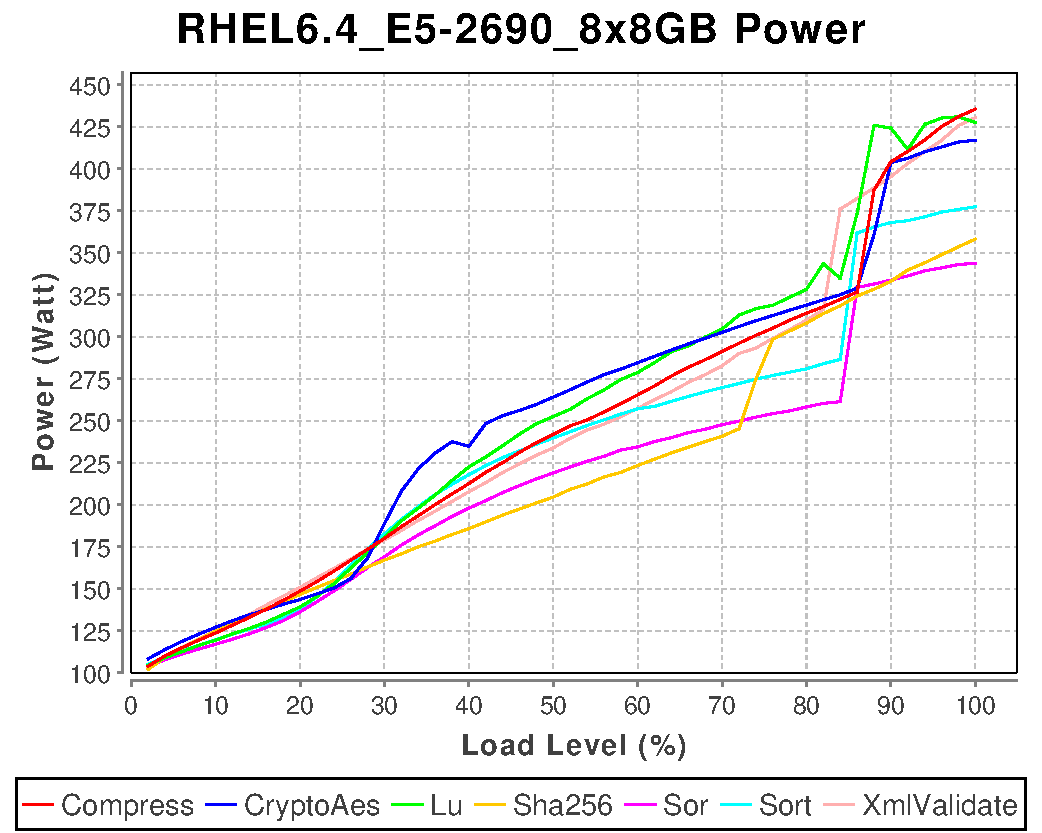
\includegraphics[trim=0cm 0cm 0cm 1cm, clip=true,width = 8.4cm]{graphics/RHEL6_4_E5-2690_8x8GB_p_truex50.pdf}
\caption{Bildunterschrift mit Zitat zur Quelle des Bildes.}
\label{fig:example}
\end{center}
%\vspace{-5mm}
\end{figure}

Im folgenden noch eine schöne Beispieltabelle (Tabelle~\ref{tab:example}):

\begin{table*}[htbp]%
	%\small
	\centering
	%\vspace{-1mm}

	\begin{tabular}{| P{2.8cm} | c :  c : c : c |}
		\hline
		\textbf{Model}        &          \textbf{Column 1}          &          \textbf{Column 2}          &          \textbf{Column 3}          &        \textbf{Column 3}        \\
		\hline
		Description 1          &              0.18\%              &             0.185\%              &             \textbf{0.149\%}              &             0.144\%              \\
		\hdashline
		Description 2 &              \textbf{0.09\%}              &             \textbf{0.143\%}              &             0.205\%              &             0.154\%              \\
		\hdashline
		Description 3    &              0.18\%              &             0.185\%              &             \textbf{0.149\%}              &             0.144\%              \\
		\hdashline
		Description 4    &             0.151\%              &             0.182\%              &             0.194\%              &             \textbf{0.127\%}              \\
		\hdashline
		Description 1    &             0.171\%              &             \textbf{0.143\%}              &             0.279\%              &             0.186\%              \\
		\hline
		Description 5  &             0.186\%              &             0.185\%              &             0.267\%              &             0.128\%              \\
		\hline
	\end{tabular}
	\caption{Caption}
	%\vspace{-5mm}
	\label{tab:example}
\end{table*}



\section{Conclusions}
\label{seq:conclusion}
Die Schlussfolgerungen beenden den Artikel und erhöhen den Abstraktionsgrad der Beschreibung wieder (hinauszoomen), genauso wie die Einleitung diesen gesenkt hat (hineinzoomen). Meist sind ``Conclusions'' sehr wichtig, da viele Gutachter nach ``Abstract'' und ``Introduction'' zunächst die ``Conclusions'' lesen und dann voreingenommen den Rest des Artikels lesen. Idealerweise bestehen die ``Conclusions'' aus den folgenden 3 Punkten, für die jeweils ein Abschnitt spendiert werden sollte:
\begin{enumerate}
	\item Zusammenfassung: Was wurde in dieser Arbeit gemacht? Was waren die Schlüsselergebnisse? Diesmal jedoch zusammengefasst nochmals für einen Leser, der die vorherigen Seiten mit allen Details bereits gelesen hat.
	\item Adressaten der Verbesserung: Wem nützen die Verbesserungen/Beiträge der Arbeit? Inwieweit wird die Software-Technik (oder Informatik als Ganzes) durch die Arbeit verbessert?
	\item Aufbauende/Zukünftige Arbeiten: Welche nächsten Schritte sind geplant (erst kurzfristige, dann längerfristige)? Welche möglichen Lösungsansätze für noch bestehende Probleme sind denkbar? Wie könnten zukünftige Forschungsarbeiten aussehen?
\end{enumerate}

%\newpage
\bibliographystyle{splncs03}
\bibliography{sesebib}

\end{document}
